  \documentclass[final]{beamer} % beamer 3.10: do NOT use option hyperref={pdfpagelabels=false} !
  %\documentclass[final,hyperref={pdfpagelabels=false}]{beamer} % beamer 3.07: get rid of beamer warnings
  \mode<presentation> {  %% check http://www-i6.informatik.rwth-aachen.de/~dreuw/latexbeamerposter.php for examples
    \usetheme{Berlin}    %% you should define your own theme e.g. for big headlines using your own logos
  }
  \usepackage[brazil]{babel}
  \usepackage[utf8]{inputenc}
  \usepackage{amsmath,amsthm, amssymb, latexsym}
  %\usepackage{times}\usefonttheme{professionalfonts}  % times is obsolete
  \usefonttheme[onlymath]{serif}
  \boldmath
  \usepackage[orientation=portrait,size=a4,scale=1.4,debug]{beamerposter}                       % e.g. for DIN-A0 poster
  %\usepackage[orientation=portrait,size=a0,scale=1.4,debug]{beamerposter}                       % e.g. for DIN-A0 poster
  %\usepackage[orientation=portrait,size=a1,scale=1.4,grid,debug]{beamerposter}                  % e.g. for DIN-A1 poster, with optional grid and debug output
  %\usepackage[size=custom,width=200,height=120,scale=2,debug]{beamerposter}                     % e.g. for custom size poster
  %\usepackage[orientation=portrait,size=a0,scale=1.0,printer=rwth-glossy-uv.df]{beamerposter}   % e.g. for DIN-A0 poster with rwth-glossy-uv printer check
  % ...
  %
  \title[Design Sprint \& Material Design]{Workshop para apresentação e aplicação dos princípios de Design Sprint e Material Design}
  \author[Mezuro]{The Mezuro Team (mezurometrics@gmail.com)}
  \institute[CCSL - IME - USP]{Centro de Competência em Software Livre, Instituto de Matemática e Estatística da universidade de São Paulo}
  \date{17 e 18 de Novembro de 2015}
  \begin{document}
  \begin{frame}{}
    %\maketitle
    \vfill
    {\veryHuge Workshop de Design Sprint e Material Design}
    \vfill
    \begin{itemize}
      \item {\large Gosta de Software Livre?}
      \item {\large Quer interagir com designers, programadores, artistas e com muitos outros especialistas?}
      \item {\large Tem interesse em conhecer uma nova forma de se estruturar, prototipar e validar ideias?}
      \item {\large O que acha de aprender junto conosco a aplicar especificações de design?}
    \end{itemize}
    \vfill
    {\large Venha participar do workshop de \textbf{Design Sprint} e \textbf{Material Design} do Centro de Competência em Software Livre do IME - USP nos dias \textbf{17} e \textbf{18} de novembro. Nele vamos todos aprender juntos estes conceitos e trocar experiências. Este \textbf{não é um evento apenas para programadores}: quanto mais diversidade entre os participantes melhores os resultados!}
    \vfill
    {\large Vamos juntos aplicar os princípios de Design Sprint sobre desafios de usabilidade no software livre Mezuro (\url{http://mezuro.org}) desenvolvido no CCSL. Com os resultados obtidos vamos então aprender como traduzir os protótipos finais em software funcional utilizando os princípios de Material Design.}
    \vfill
    \begin{block}{\large Data e Local}
      \begin{center}
        \textbf{Auditório do CCSL (IME - USP)}
      \end{center}

        O evento será dividido em dois dias:

        \begin{itemize}
          \item \textbf{Design Sprint}: 17 de novembro das 08h às 14h
          \item \textbf{Material Design}: 18 de novembro das 13h às 18h
        \end{itemize}

        Para ter uma experiência completa programe-se para participar dos dois dias!
    \end{block}
    \begin{minipage}{0.482\linewidth}
      \begin{block}{\large Como chegar?}
        \center
        \begin{figure}[h]
          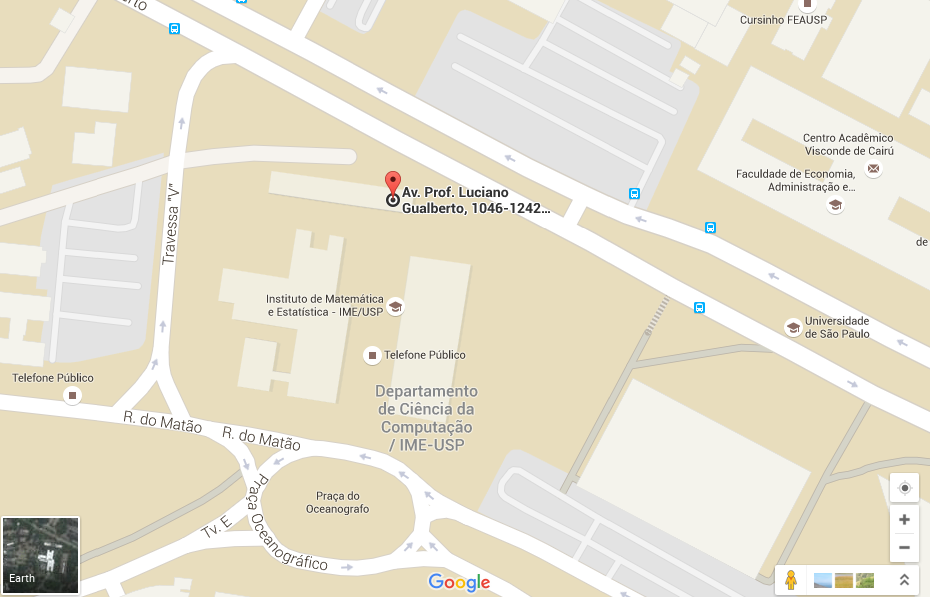
\includegraphics[height=100px]{ccsl-location}
        \end{figure}
        R. do Matão, 1010. Prédio do CCSL.
      \end{block}
    \end{minipage}
    \begin{minipage}{0.49\linewidth}
      \begin{block}{\large Inscrições pelo formulário}
        \center
        \begin{figure}[h]
          
\includegraphics[height=100px]{design_sprint_form_qr}
        \end{figure}

        \url{http://goo.gl/forms/xnOQVMfKoV}
      \end{block}
    \end{minipage}
    \vfill
    \begin{block}{\large Design Sprint}
      O sprint é um processo para fornecer respostas a questões criticas de negócio através de design, prototipação e testando ideias com usuários. Desenvolvido pela Google Ventures, é uma das metodologias da moda em estratégia de negócios, inovação, ciência comportamental, \textit{design thinking}, e mais — empacotado em um processo que qualquer time pode usar.

      Mais detalhes em: \url{http://www.gv.com/sprint/}
    \end{block}
    \vfill
    \begin{block}{\large Material Design}
      A Google se desafiou a criar uma linguagem visual para seus usuários que sintetize os princípios clássicos do bom design com inovação e as possibilidades da tecnologia e ciência. Como resposta a este desafio foi produzida a especificação \textit{Material Design} com três princípios:

      \begin{itemize}
        \item Material é a metáfora
        \item Ousado, gráfico e explícito
        \item Movimento fornece significado
      \end{itemize}

      Mais detalhes em: \url{https://www.google.com/design/spec/material-design/introduction.html}
    \end{block}
    \vfill
    {\large Quaisquer dúvidas entre em contato por: mezurometrics@gmail.com}
    \vfill
  \end{frame}
\end{document}
